
\documentclass[11pt,a4paper]{article}

\usepackage[utf8]{inputenc} 
\usepackage[T1]{fontenc} 
\usepackage{lmodern}
\usepackage{tcolorbox}
\usepackage[german]{babel}

\usepackage{fourier}
\setlength{\parindent}{0pt}
\setlength{\parskip}{1ex plus 0.5ex minus 0.5ex}

\usepackage{amsmath} 


\usepackage{graphicx} 

\usepackage[section]{placeins}
\usepackage{booktabs}


\usepackage{hyperref}
\hypersetup{
	colorlinks,
	citecolor=red,
	filecolor=black,
	linkcolor=black,
	urlcolor=black}
\graphicspath{}

\begin{document}
	

{
	\centering 
	\large 
	Physiklabor für Anfänger*innen \\
	Ferienpraktikum im Sommersemester 2018 \\[4mm]
	\textbf{\LARGE 
		Versuch 14: Streuversuch
	} \\[3mm]
	(durchgeführt am 05.10.2018 bei Assistentin Julia Müller) \\
	Ye Joon Kim, Marouan Zouari\\
	\today \\[10mm]
}

\tableofcontents
\section{Einleitung}



\section{Aufbau}
Der Aufbau dieses Versuchs besteht aus einem großen Hohlzylinder mit einem kleineren Hohlzylinder in der Mitte. Auf einer Seite des großen Zylinders gibt es eine Öffnung, wodurch die kleine Kugeln mit einem verschiebbaren Luftdruckkugelbeschleunigungsgerät geschossen werden können. Die innere Seite des Zylinders wurde mit druckempfindlichem Papier gelegt (Siehe Abbildung 1). Es wurden auch einen Lineal und Maßband verwendet. 

\section{Durchführung}
Zuerst wurde der Durchmesser des Innenraums des großen Hohlzylinders mit einem Maßband gemessen. Die Position $\theta = 0$ wurde auch mit dem Maßband bestimmt und auf das Papier markiert. Das Kugelschießgerät wurde dann so verschoben, sodass die geschossenen Kugel zurückreflektiert werden. Die Position des Geräts wurde dann als $b_0$ aufgenommen. Das Gerät wurde danach nach rechts verschoben, ihre Position aufgenommen und mit 20 Kugeln geladen. Die Kugel wurden dann mithilfe des Ballonförmigen Bauteils geschossen. Die Markierungen auf dem Paper wurde dann gekennzeichnet. Dieser Prozess wurde für acht andere Positionen des Geräts auf beide Seiten des Targetzylinders wiederholt. Das druckempfindliche Papier wurde dann entnommen und die mittleren Positionen der Markierungen sowie deren Streuung abgeschätzt und auf dem Papier gezeichnet. 


\section{Auswertung und Fehleranalyse}

Die Werte für $b$ und der Mittelwerte von $\widearc{AB}$ sowie deren Unsicherheiten sind in Tabelle 1 zu sehen.


\begin{table}[h]
	\centering
	\begin{tabular*}{0.50\textwidth}{@{\extracolsep{\fill}}ccccc}
		\toprule
		$b$ & $\Delta b$ & $\overline{\widearc{AB}}$ & $s_{\widearc{AB}}$ & $u_{\overline{\widearc{AB}}}$ \\
		cm & cm & cm &cm& cm\\
		\midrule
		-0,5 & 0,1 & -89,3 & 0,4 & 0,2\\
		-0,8 & 0,1 & -84,7 &0,6& 0,2\\
		-1,2 & 0,1 & -76,6 &0,6& 0,2\\
		1,2 & 0,1& 78,9 &0,9& 0,2 \\
		1,7 & 0,1 & 67,0 &1,3& 0,3 \\
		2,2 & 0,1 & 53,2 &1,2& 0,3 \\
		-1,8 & 0,1 & -59,7 &1,3& 0,3 \\
		2,7 & 0,1 & 37,9 &1,4& 0,3\\
		\bottomrule
\end{tabular*}
\caption{Die gemessenen Werte für $b$, $\overline{\widearc{AB}}$ und deren Unsicherheiten}
\end{table}

\begin{tcolorbox}[colback=white]
\subsection{Rechenweg}
Für die Unsicherheit von $b$ wurde die vereinfachte gaußsche Fehlerfortpflanzung benutzt. Da $b$ sich um eine Differenz handelt, ist:
$$\Delta b = \sqrt{(\Delta b_n)^2 + (\Delta b_0)^2}$$

Für die Unsicherheiten von $\overline{\widearc{AB}}$ wurde die abgeschätzten Standardabweichungen durch einen Faktor $\sqrt{n}$ geteilt, da es geht um einen Mittelwert. Es wurden auch die Ablesefehler von $\widearc{AB}$ und von dem Punkt $A$ berücksichtigt. Deswegen beträgt der gesamte Fehler von $\overline{\widearc{AB}}$:
$$
u_{\overline{\widearc{AB}}} = \sqrt{\left(\frac{s_{\widearc{AB}}}{\sqrt{n}}\right)^2+u_\textrm{Ab}^2+u_A^2}
$$
In diesem Fall waren $u_\textrm{Ab}$ und $u_A$ beide 0,1 cm.
\end{tcolorbox}

Danach wurde die $\overline{\widearc{AB}}$ Werte in $\theta$ umgewandelt (Siehe Tabelle 2).

\begin{table}[h]
	\centering
	\begin{tabular*}{0.50\textwidth}{@{\extracolsep{\fill}}cccc}
		\toprule
		$b$ & $\Delta b$ & $\theta$ & $u_\theta$  \\
		cm & cm & rad & rad \\
		\midrule
		-0,5 & 0,1 & -2,812 & 0,005\\
		-0,8 & 0,1  &-2,668& 0,005\\
		-1,2 & 0,1  &-2,413& 0,005\\
		1,2 & 0,1 &2,485& 0,007\\
		1,7 & 0,1  &2,11& 0,01\\
		2,2 & 0,1  &1,68& 0,01\\
		-1,8 & 0,1  &-1,88& 0,01\\
		2,7 & 0,1  &1,19& 0,01\\
		\bottomrule
	\end{tabular*}
\caption{Die Werte für $\theta$ und ihre Unsicherheiten}
\end{table}

\begin{tcolorbox}[colback=white]
\subsection{Rechenweg}
Da $\theta = \frac{\widearc{AB}}{R}$, wurde die vereinfachte gaußsche Fehlerfortpflanzung für Produkte verwendet, deswegen ist
$$ \left|\frac{u_\theta}{\theta}\right| = \sqrt{\left(\frac{u_{\widearc{AB}}}{\widearc{AB}}\right)^2+\left(\frac{\Delta r}{r}\right)^2}$$
\end{tcolorbox}

Die Werte für $\cos{\frac{\theta}{2}}$ wurden dann gegen $b$ aufgetragen (Siehe Abbildung 2). 
\begin{figure}[h]
	\centering
	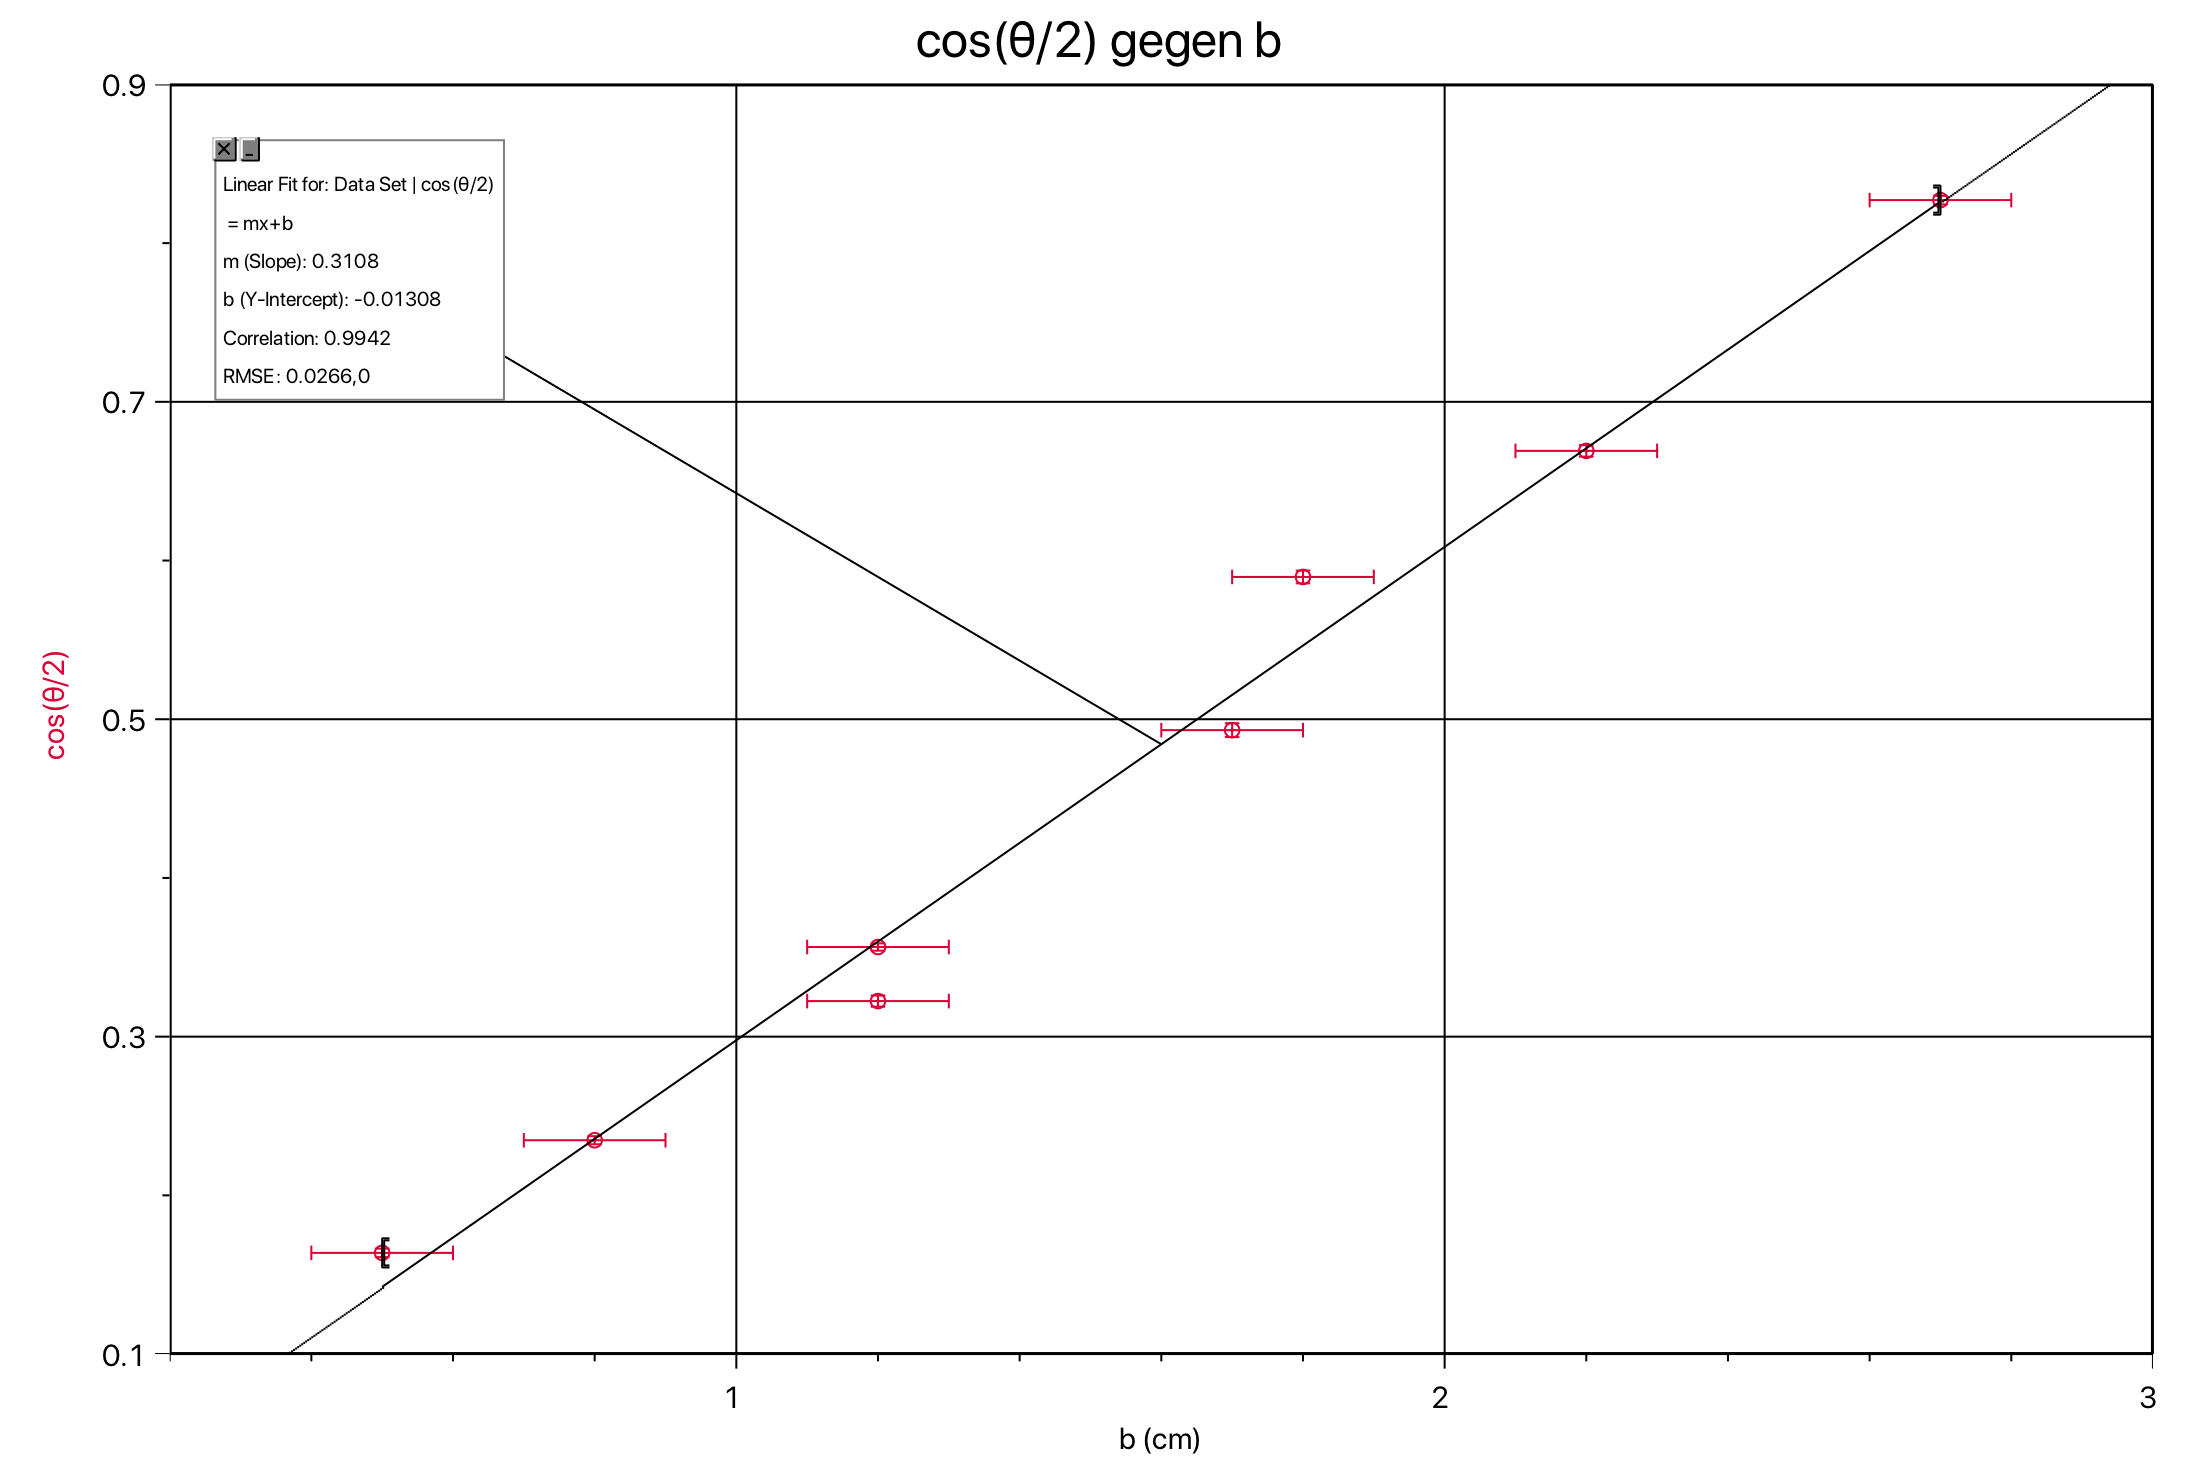
\includegraphics[width=\linewidth]{Abb2}
	\caption{Eine Auftragung von $\cos{\frac{\theta}{2}}$ gegen $|b|$}
\end{figure}

Da $\cos{\frac{\theta}{2}}$ linear zu $b$ ist, kann der Zusammenhang dazwischen in so einer Form:
$$ \cos{\frac{\theta}{2}} = a+m\cdot b$$
geschrieben werden. $m$ entspricht deshalb dem Wert $\frac{1}{r+R}$. Die Werte und Unsicherheiten für $a$ und $b$ wurden mit einem Excel-Dokument berechnet:
$$ a = (-0,01 \pm 0,02) $$
$$ m = (0,31 \pm 0,01) \textrm{s}^{-1} $$

\begin{tcolorbox}[colback=white]
\subsection{Rechenweg}
Obwohl in der Abbildung unsichtbar, wurden die Unsicherheiten der $\cos{\frac{\theta}{2}}$ mit der gauß'schen Fehlerfortpflanzung berechnet. 
Mit:
$$f(\theta) = \cos\frac{\theta}{2}$$
ist
$$\frac{\partial f}{\partial \theta} = -\frac{1}{2}\sin\frac{\theta}{2}$$
Deshalb ist die Unsicherheit:
$$u_{\cos\frac{\theta}{2}} = \frac{\partial f}{\partial \theta}\cdot u_\theta$$

Für die Bestimmung der Werte und Unsicherheiten für $a$ und $m$ wurden die folgenden Formel benutzt:
$$a = \frac{
	\sum x_i^2 \sum y_i - \sum x_i \sum x_iy_i
}{
	n \sum x_i^2 - (\sum x_i)^2
}$$
$$ m = \frac{
	n\sum x_iy_i-\sum x_i \sum y_i
}{
	n \sum x_i^2 - (\sum x_i)^2
}$$

$$u_a = s\cdot \sqrt{
	\frac{
		\sum x_i^2
	}{
		n\sum x_i^2 - (\sum x_i)^2
}}$$

$$u_m = s\cdot \sqrt{
	\frac{
		n
	}{
		n\sum x_i^2 - (\sum x_i)^2
}}$$
Mit $x = b$, $y = \cos\frac{\theta}{2}$ und $s = \sqrt{
	\frac{1}{n-2}\sum [y_i-(a+mx_i)]^2}$
	
\end{tcolorbox}

Jetzt kann der Wert für $R$ mit der Steigung $m$ berechnet werden:
$$ R = {3,0 \pm 0,1} \textrm{cm} $$

\begin{tcolorbox}[colback=white]
\subsection{Rechenweg}
Der $R$ Wert 


Für die Berechnung der Unsicherheit wurde die Gaußsche Fehlerfortpflanzung benutzt. Mit
$$R(m) = \frac{1}{m}-r$$ 
ist
$$\frac{\partial R}{\partial m} = -\frac{1}{m^2}$$
Die Unsicherheit von $R$ ist deshalb:
$$u_R = \left|\frac{\partial R}{\partial m}\cdot u_m\right|$$

	
\end{tcolorbox}


\end{document}
